%-----------------------------------------------------------------------------
%
%    Domain Specific Identifiers
%
%-----------------------------------------------------------------------------


%\documentclass[preprint,authoryear]{acm_proc_article-sp}
%\documentclass{acm_proc_article-sp}
%\documentclass[preprint,authoryear]{acm_proc_article-sp}
%\documentclass[preprint,authoryear,10pt]{sigplanconf}

\documentclass[preprint]{sigplanconf}

\usepackage{csvsimple}
\usepackage{ifthen}
\usepackage{pifont}
%\usepackage[small,compact]{titlesec}

% \usepackage{mathptmx}

% \usepackage{paralist}

% \usepackage[small,it]{caption}

\usepackage[pdftex]{graphicx}


%\usepackage{fancyhdr}


\usepackage{amsmath}
\usepackage{epigraph}
\usepackage[colorlinks=true,
        linkcolor=blue,
        citecolor=red,
        filecolor=black,
        urlcolor=black,
        bookmarks=true,
        bookmarksopen=true,
        bookmarksopenlevel=3,
        plainpages=false,
        pdfpagelabels=true]{hyperref}

%%--- listings configuration
\usepackage{listings}
\lstset{
  language={C},
  basicstyle=\ttfamily,
  keywordstyle=\bfseries,
  showstringspaces=false,
  commentstyle=,
  captionpos=below%,
%  numbers=left,
%  numberstyle=\tiny,
%  numbersep=5pt
}
\lstset{numberbychapter=false}

%\lstdefinestyle{L}{basicstyle=\ttfamily}
\lstdefinestyle{L}{basicstyle=\ttfamily\scriptsize}
\lstdefinestyle{numbers}
{numbers=left, stepnumber=1, numberstyle=\tiny, numbersep=10pt,basicstyle=\ttfamily\scriptsize}

%%--- end of listings configuration

%\pagestyle{fancy} 
% \sloppy

%\setlength{\parskip}{0pt}
%\setlength{\parsep}{0pt}
%\setlength{\headsep}{2pt}
%\setlength{\topskip}{0.1pt}
%\setlength{\topmargin}{1pt}
%\setlength{\topsep}{1pt}
%\setlength{\partopsep}{0pt}

\newboolean{showcomments}
\setboolean{showcomments}{true}



\ifthenelse{\boolean{showcomments}}
  {\newcommand{\mynote}[2]{
      {\color{red}
    \fbox{\bfseries\sffamily\scriptsize#1}
%       {\small$\blacktriangleright$\textsf{\emph{#2}}$\blacktriangleleft$}
       {\small \textsf{\emph{#2}} }
    % \marginpar{\fbox{\bfseries\sffamily#1}}
        }
   }
   \newcommand{\cvsversion}{\emph{\scriptsize $ $Revision: 1.42 $ $ -- $ $Date: 2005/10/01 00:23:32 $ $ }}
  }
  {\newcommand{\mynote}[2]{}
   \newcommand{\cvsversion}{}
  }

\newcommand{\here}{\mynote{***}{CONTINUE HERE}}
\newcommand\nb[1]{\mynote{NB}{#1}}
\newcommand\fix[1]{\mynote{FIX}{#1}}
% \newcommand\todo[1]{\mynote{TO DO}{#1}}
\newcommand\mpw[1]{\mynote{Marcel}{#1}}
\newcommand\rh[1]{\mynote{Robert}{#1}}

%\renewcommand{\topfraction}{0.85}
%\renewcommand{\textfraction}{0.1}
%\renewcommand{\floatpagefraction}{0.85}



\begin{document}
%\fontsize{9.7}{12}\rm

%\linespread{0.9}

\conferenceinfo{SPLASH 2013}{date, City.} 
\copyrightyear{2013} 
\copyrightdata{[to be supplied]} 

%\titlebanner{banner above paper title}        % These are ignored unless
%\preprintfooter{short description of paper}   % 'preprint' option specified.


\title{Uniform Resource Access in Objective-Smalltalk with Polymorphic Identifiers}

%\author{Marcel Weiher\inst{1} \and Robert Hirschfeld\inst{2}}
%\institute{metaobject ltd. \email{marcel@metaobject.com} \and Hasso Plattner Institut \email{robert.hirschfeld@hpi.uni-potsdam.de}}


\authorinfo{Marcel Weiher}
           {metaobject ltd.}
           {marcel@metaobject.com}
\authorinfo{Robert Hirschfled}
           {Hasso Plattner Institut}
           {hirschfeld@acm.org}

%\numberofauthors{2}
%\author{
%\alignauthor Marcel Weiher\\
%       \affaddr{metaobject ltd.}\\
%       \email{marcel@metaobject.com}
%\alignauthor Robert Hirschfeld\\
%       \affaddr{Hasso Plattner Institut}\\
%       \email{}
%}

\maketitle

\begin{abstract}

In object-oriented programming, polymorphic dispatch of operations
decouples clients from specific providers of services and allows 
implementations to be modified or substituted without affecting clients. 

The Uniform Access Principle (UAP) tries to extend these qualities to 
resource access by demanding that access to state be indistinguishable
from access to operations.  Despite language features supporting the
UAP, the overall goal of substitutability has not been achieved for
either alternative resources such as keyed storage, files or web pages, or for alternate 
access mechanisms:    
specific kinds of resources are bound to specific access mechanisms and vice versa.
Changing storage or access patterns either requires changes to both clients and
service providers and trying to maintain the UAP imposes significant penalties in terms of
code-duplication and/or performance overhead.

We propose introducing first class identifiers as polymorphic names for storage locations
to solve these problems.  With these \emph{Polymorphic Identifiers}, we show that
we can provide uniform access to a wide variety of resource types as well as 
storage and access mechanism, whether parametrized or direct, without affecting
client code, without causing code duplication and improving performance significantly.

\end{abstract}

% \category{D.3.3}{Programming Languages}{Language Constructs and Features}

%\terms{language, design}
%\keywords{Polymorphic Identifiers} % NOT required for Proceedings
%\setlength{\epigraphrule}{0pt}

%-=-=-=-=-=-=-=-=-=-=-=-=-=-=-=-=-=-=-=-=-=-=-=-=-=-=-=-=-=-=-=-=-=-=-=%

\section{Introduction}

Imperative object oriented languages such as Smalltalk, C\#, Java or Objective-C provide
built-in storage for their objects in the form of instance variables.  These instance
variables 

Imperative programming languages such a Pascal or C clearly distinguish between
data access and procedure or function invocation at the language level.  Data 
access is via \emph{L-Values}, that is \emph{Locations} that point into a \emph{store}~\cite{StracheyFund}
and can be read or written, whereas procedures and functions can only be invoked.

\begin{itemize}
\item only one kind of state, others via procedural abstraction (I/O, hash-table, ...)
\item early OOP still has that distinction
\item conflicts with representation independence, so UAP
\item implementations of UAP:  remove state access / properties
\item Problem:  still not enough, state variants leak
\item 
\end{itemize}


Imperative programming languages feature the concept of a store with locations.
Locations or \emph{L-Values} are characterized by the essential features of having content 
(an associated R-Value) and 2 operations to access and update this value from the location,
the \emph{Load-Update-Pair} or \emph{LUP} (also Strachey).  Strachey decouples the definition of a store
from the notion of memory or addressability. 

The same goes for parametrized access via pointers, which are 
R-Values that represent locations.  Pointers are characterized by two polymorphic 
operations, \emph{Follow} and \emph{Pointer}.  

Programming languages such as Pascal or C implement the store as main memory, with
identifiers mediating access.  We can compose these identifiers, use them on the LHS and RHS
and partially use them for indirect access.  Computational abstraction is handled separately.

Object-oriented programming languages mostly maintain the distinction between computational
and storage abstraction, with polymorphism and most other abstraction mechanisms only
applying to computational abstraction.  The better support for abstraction afforded by 
the computational abstraction mechanism has led to storage abstraction being 
de-emphasized by convention (Java, C\#,..) or by removing it partially (Smalltalk) or 
entirely (Self, Newspeak) from the user-visible language, reducing the number
of concepts in the language.  



The Uniform Access Principle (UAP) was coined by Meyer to formalize this relationship:  
access to state should be indistinguishable from computation.  However, the current
implementations interpret this as applying only to state in instance variables of objects.






%-=-=-=-=-=-=-=-=-=-=-=-=-=-=-=-=-=-=-=-=-=-=-=-=-=-=-=-=-=-=-=-=-=-=-=%





\section{Non-uniform access}
\label{nonuniform}
%\epigraph{When programming a component, the right computation model for the component is the least expressive model that results in a natural program.}{Rule of Least Expressiveness.}

This section provides three resource access scenarios where uniform access is difficult to achieve
with standard mechanisms, leading to compromises and non-uniform access patterns in practical
code.  Please note that this section is not about exhaustively enumerating all possible solutions
or conclusively proving that no better solutions exist. Instead it highlights that for common and
simple situations, achieving the goals of the UAP is not necessarily simple and obvious, and
non-uniform solutions are often viable and commonly used alternatives.

\begin{table}
\center
\begin{tabular}{|l|c|c|} \hline
   & C\#  	 & Objective-C  		 \\\hline 
read property & {\tt c = a.b; }	 & {\tt c = a.b;  }		 \\\hline 
write property & {\tt a.b = c; }	 & {\tt a.b = c; }		 \\\hline 
send message & {\tt a.b(c);  }	 & { [a b:c]; }		 \\\hline 
\shortstack{{define property}\\{autogenerated}}  & \shortstack{ {\tt public int b} \\ { \{\tt get; set; \} }}  & \shortstack{{\tt @property int b;}\\{\tt @synthesize b;}}\\\hline 
\end{tabular}
\caption{C\# and Objective-C syntax}
\label{objc-syntax}
\end{table}

We use Objective-C in our examples because it has both properties and a ``message not understood''
hook for handling messages without implementing them.  Table~\ref{objc-syntax} shows basic
Objective-C syntax compared to C\#.  


\subsection{User-defined storage implementations}
\label{userdefined}
Although language features supporting the UAP make it easy to substitute a single 
instance variable with a pair of methods or vice versa, substituting custom stores,
and doing so wholesale, is more difficult.

For our examples, we will be using a trivial {\tt Person} class shown in Listing~\ref{personclassdef}
using Objective-C syntax with property definitions for attributes {\tt name} and {\tt age}.

\begin{figure}[htbp]
\begin{lstlisting}[style=numbers,label=personclassdef,caption=Person class.]
@interface Person : NSObject 
{}
@property NSString *name;
@property NSNumber *age;
...@end
@implementation Person
@synthesize name,age, ...;
@end
\end{lstlisting}
\end{figure}


Dictionaries provide a generic interface to access their contents, so they have
one method for retrieving objects by key and another method for storing objects
by key, in our example {\tt objectForKey:} and {\tt setObject:forKey:} whereas
object properties can be accessed using dot notation and the property name.
Listing~\ref{dict-vs-property1} summarizes the differences, it is clear that implementations
cannot simply be substituted as is.


\begin{figure}[htbp]
\begin{lstlisting}[style=numbers,label=dict-vs-property1,caption=Dictionary vs. Property.]
person.name;
person.name = newName;
person[@"name"];
person[@"name"] = newName;
\end{lstlisting}
\end{figure}

It should be noted that similar to C\# and Eiffel, the syntax in  Listing~\ref{dict-vs-property1}
is surface syntax only that is mapped by the compiler to the message sends shown in
Listing~\ref{dict-vs-messages}.  

\begin{figure}[htbp]
\begin{lstlisting}[style=numbers,label=dict-vs-messages,caption=Dictionary vs. Property.]
[person name];
[person setName:newName];
[person objectForKey:@"name"];
[person setObject:newName forKey:@"name"];
\end{lstlisting}
\end{figure}

There are three basic options for bridging the gap and making access uniform between the
dictionary and the object:
\begin{enumerate}
\item  Listing~\ref{compatibility1} adapts the object to the dictionary's protocol by
	 implementing {\tt objectForKey:} and {\tt setObjectForKey:} and mapping the keys
	 to properties.
\item Listing~\ref{compatibility2} adapts the dictionary to the object's protocol by 
	implementing cover methods for every potential attribute that is to be stored.
\item Listing~\ref{compatibility3} also adapts the dictionary to the object's protocol, but
	this time by implementing the "forwardInvocation:" error handler that is invoked
	when a message is not understood by an object.
\end{enumerate}

None of these options is particularly appealing, as they all involve either performance penalties,
repetitive code or both.
	
\begin{figure}[htbp]
\begin{lstlisting}[style=numbers,label=compatibility1,caption=Making an object dictionary-compatible.]
-objectForKey:aKey
{
  if ( [aKey isEqual:@"name] ) {
    return self.name;		
  } else if ( [aKey isEqual:@"age] ) {
    return self.age;
  } else if ...
  }
}
-setObject:newObject forKey:aKey 
  if ( [aKey isEqual:@"name] ) {
    return self.name=newObject;		
  } else if ( [aKey isEqual:@"age] ) {
    return self.age=newObject;
  } else if ...
  }
}
\end{lstlisting}
\end{figure}

Adopting the dictionary's protocol as in Listing~\ref{compatibility1} as the uniform interface between
clients and their service providers means 
that the language's built in notations for access will no longer be used for interfacing between
objects, rather {\tt objectForKey:} and {\tt setObject:forKey:} will now be used universally.  In addition
to bloating client code and making it virtually unreadable, this also means having to implement
the {\tt objectForKey:}/{\tt setObject:forKey:} methods for every object.  These methods are not just
boilerplate that duplicates the already-existing property definitions, they are also more than an order
of magnitude slower than the built-in access, and slower even than dictionary access.  This 
performance overhead is imposed by the API, it cannot easily be removed by clever implementations.

In combination, these aspects of this solution strongly discourage object-modeling, as just using 
dictionaries everywhere is not just less code, but also faster than introducing objects.

\begin{figure}[htbp]
\begin{lstlisting}[style=numbers,label=compatibility2,caption=Making a dictionary object-compatible.]
-(NSString*)name
{
    return [self objectForKey:@"name];
}
-(void)setName:(NSString*)newName
{
  [self setObject:newName forKey:@"name];
}
-(NSNumber*)age
{
    return [self objectForKey:@"age"];
}
-(void)setAge:(NSNumber*)newAge 
{
  [self setObject:newName forKey:@"age"];
}
...
\end{lstlisting}
\end{figure}

The second option is to keep property access as the universal interface, mapping to dictionaries
inside the object using cover methods as shown in Listing~\ref{compatibility2}.  The advantages
of this approach are that we do no abandon the language-defined interface facilities and
there is no performance overhead imposed by the API.  The disadvantage is obvious from
Listing~\ref{compatibility2}:  introduction of duplicated boilerplate code on a massive scale.

Although independent identifiable concerns are supposed to be isolated in a single module~\cite{Parnas72},
and object-orientation is supposed to help us with this goal,
this ``storage concern'' is now spread all over the code-base.  If we want to change storage
from instance variables to dictionaries or back for a variety of objects, we must modify all
the objects involved, introducing or removing these cover methods as needed. 


\begin{figure}[htbp]
\begin{lstlisting}[style=numbers,label=compatibility3,caption=Compatibility via forwardInvocation.]
-(void)forwardInvocation:(NSInvocation*)inv 
{
  SEL sel=[inv selector];
  NSString *msg=NSStringFromSelector( sel );
  if ( [msg hasPrefix:@"set"] ) {
    NSRange  r      = NSMakeRange(3,1);
    NSString *first = [msg substringWithRange:r];
    NSString *rest  = [msg substringFromIndex:4];
    NSString *key   = nil;
    id arg=nil;
    [inv getArgument:&arg atIndex:2];
    first=[first lowercaseString];
    key=[first stringByAppendingString:rest];
    [self setObject:arg forKey:key];
  } else {
    id result=[self objectForKey:msg];
    [inv setResult:&result];
  }
}
...
\end{lstlisting}
\end{figure}

In dynamic languages, we have a third option, using the error handler invoked when a method
is not found to simulate the cover methods without having to implement them, as shown
in Listing~\ref{compatibility3}.   Although this approach does reduce the need to write
cover methods for each individual attribute, it still needs to be implemented for every keyed
access class or injected if injection facilities are available.  The fact that it must convert
distinct message message names to keys via string processing not only makes it fragile,
but also quite slow, at around three orders of magnitude slower than a plain message
send accessing an attribute.

Although we have shown three possible ways of honoring the UAP when dealing with custom
attribute storage in Objective-C, all of them come with
serious drawbacks, and so the fourth, not previously listed option is usually chosen:  simply
live with non-uniform access for custom stores.

Other object-oriented languages such as C\#, Scala, Python, Ruby, Eiffel, Java and Smalltalk,
present the developer with the same tradeoffs, though details vary slightly and the dynamic
message resolution technique from Listing~\ref{compatibility3} is only available in the dynamic
languages. 

The problems presented apply to any custom store, not just dictionaries,
because any custom store has to identify the storage locations (\emph{L-Values}) to reference,
so it has to translate from messages to \emph{L-Values} and back somehow.  Furthermore,
they are transitive:  they apply just as much if we hide a custom store inside of an object as
they do when we substitute the custom store directly for the object.

  Special 
machinery is sometimes available to perform this translation for instance variables (in the form of 
properties in C\#, Python and Objective-C, in the form of aliases in Eiffel and Scala and hidden
in Self), but these mechanism only apply to instance variables, not to custom stores.



\subsection{Parametrized access}
\label{parametrized}
Another source of non-uniformity is the difference between direct access, where the attribute
to be accessed is known at compile time and present in the source code, and parametrized
access, where the exact attribute is passed as a parameter at run time.  Parametrized access
is frequently used in UI toolkits, serialization and persistence mechanisms in order to generically
access attributes of an object.  For example, a
UI text field is parametrized in order to be able to read and write the {\tt name} attribute of
an object.

Table~\ref{direct-vs-parametrized}
summarizes how read and write access to an attribute differs between direct and parametrized
access in Objective-C.  Property access is the simplest, as there simply is no parametrized variant
available.  Keyed access can use the same message format for indirect and direct access, and
more crucially, the same key for both read and write access.  Message-based access, on the
other hand, must not only switch from the direct messaging syntax to indirect {\tt perform:}
messages, but also must provide two different message selectors, the read and the write
selector (e.g. {\tt name} and {\tt setName:}).

\begin{table*}[htbp]
\center
\begin{tabular}{|r|c|c|} \hline
   &  direct	 & parametrized  		 \\\hline 
property read 	 &   {\tt person.name;  }	&  -	 \\\hline 
property write 	 & {\tt person.name=newName; }	 & -		 \\\hline 
message read 	 &  {\tt  [person name]; }	 & {\tt [person perform:readAttrSel]; }		 \\\hline 
message write 	 & {\tt  [person setName:newName]; }	 & {\tt [person perform:writeAttrSel with:newName]; }		 \\\hline 
keyed read  & {\tt person[@"name"]; }	 & {\tt person[anAttribute];  }  \\\hline 
keyed write  & {\tt person[@"name"]=newName;}	 & {\tt person[anAttribute]=newName; }		 \\\hline 
\end{tabular}
\caption{Direct vs. parametrized access}
\label{direct-vs-parametrized}
\end{table*}


In order to have parametrized read/write access to an attribute, we again seem to have effectively
three options:

\begin{enumerate}
\item Use dictionaries or another keyed store exclusively when parametrized access is required
\item Map a keyed API to message-sends dynamically (option 2 of section~\ref{userdefined}).
\item Implement an ``L-Value Reference'' object that either captures or dynamically derives 
	the two message required to access the specified attribute relative to an object.
\end{enumerate}


Option 1 leads to either non-uniform access or standardizing on dictionaries and foregoing 
object-oriented modeling.   It also means that even direct access, with all values known
at compile-time, must use the same run time access path, with the order-of-magnitude
performance penalty.
 
Option 2 is an option, but due to the negative performance
consequences we looked at in
section~\ref{userdefined} not a good one.   Option 3,  performing the computation of the selectors
in an object and reusing that object has the potential of being much faster. 

\begin{figure}[htbp]
\begin{lstlisting}[style=numbers,label=valueaccessor,caption=Class encapsulating message-based attribute access.]
@interface ValueAccessor : MPWObject
{
  id target;
  NSString *attributeName;
  SEL         getSelector,putSelector;
}
@property (strong) NSString *attributeName;
-initWithTarget:aTarget attribute:(NSString*)attrName;
-value;
-(void)setValue:
@end
@implementation ValueAccessor
@synthesize attributeName;
-initWithTarget:aTarget attribute:(NSString*)attrName
{
  self=[super init];
  getSelector=NSSelectorFromString( attrName );
  NSString *setName=[attrName capitalizedString];
  setName=[setName stringByAppendingString:@":"];
  setName=[@"set" stringByAppendingString:setName];
  putSelector=NSSelectorFromString( setName );
  return self;
}
-value
{
  return [self perform:getSelector];
}
-(void)setValue:newValue
{
  [self perform:setSelector with:newValue];
}
\end{lstlisting}
\end{figure}

A {\tt ValueAccessor} class implementing this idea is shown in Listing~\ref{valueaccessor}.  However, 
as demonstrated in Listing~\ref{valueaccessoruse}, using this
{\tt ValueAccessor} class is significantly more verbose and less convenient than just using the 
direct keyed access method of option 2.  This means that it is unlikely to be used in a direct-use
setting, so transformation from direct to parametrized use implies a large change in client code.

In addition, we have to take into account the findings from
section~\ref{userdefined}, which concluded that we are likely to not have uniform access based on
messages only, which option 3 relies on.  

\begin{figure}[htbp]
\begin{lstlisting}[style=numbers,label=valueaccessoruse,caption=Keyed access vs. using a ValueAccessor]
id valueAccessor = [[ValueAccessor alloc]
           initWithTarget:person 
           attributeName:@"name"];
a = [valueAccessor value];
\end{lstlisting}
\end{figure}

Again, we find that although we have several solutions that offer different trade-offs, no obvious
method presents itself for achieving uniformity of access when parametrized access is involved.
In fact the problems of not having uniform direct access compound the problems of parametrized access.


\subsection{External resources}

Interaction with resources outside the application's memory space keeps increasing
in importance,
for example Apple's Pages DTP application has 3.9MB of compiled code,
but 250MB of non-code resources in 18792 files (not counting frameworks), and
mobile applications are often just thin wrappers around web-resources accessible
via HTTP~\cite{http}.  However, API and language support
for abstracting over such resources is limited.  In a way that is similar to the custom stores we looked at in section~\ref{userdefined}, languages make it difficult to create APIs that separate concerns
and respect the UAP.

Listing~\ref{imagefromfile} shows loading an image file from a file using a convenience
API.   An instance of the {\tt NSBitmapImageRep} class is initialized by reading the file
from the absolute file-system path {\tt /Users/john/button.png}.

\begin{figure}[htbp]
\begin{lstlisting}[style=numbers,label=imagefromfile,caption=Accessing an image from the file system]
image = [[NSBitmapImageRep alloc] 
        initWithContentsOfFile:@"/Users/jo/button.png"];
\end{lstlisting}
\end{figure}

Rather than hiding implementation details and allowing
 them to be varied independently, the API used in Listing~\ref{imagefromfile} requires the caller
to expose and determine virtually all implementation details right at the call site:

\begin{enumerate} 
\item The fact that we are loading data from a filesystem
\item The name of the image and the full access path to the image, encoded as a literal string, so
	the API assumes that strings are filesystem paths
\item The fact that the image is encoded in the PNG file format
\item The class that will be used to represent the image in code
\end{enumerate}

If we wish to separate the resource name from its access path, we need to do string 
processing to combine the two back into a full path.  Using relative paths is dangerous
at best because those are relative to the current working directory, which is global to
the process and not necessarily predictable.

If we wish to load the image from the web rather than from the local filesystem, we need to
change APIs, as shown in Listing~\ref{imagefromweb}.  Being URI-based, the
API in this example can also be used to load images from the filesystem, but its additional
complexity and verboseness make the previous convenience API preferable as long as
it is sufficient.

\begin{figure}[htbp]
\begin{lstlisting}[style=numbers,label=imagefromweb,caption=Loading image from web]
uristring = @"http://example.com/button.png"
imaguri = [NSURL URLWithString:uristring];
data = [NSData dataWithContentsOfURI:imageuri];
image = [[NSBitmapImageRep alloc] initWithData:data];
\end{lstlisting}
\end{figure}

Similarly, if we decide to use a vector file format such as PDF, we need to change the
class to {\tt NSPDFImageRep} and the file name.  Finally, if we decide to create the
image programmatically rather than loading it from a file, we must change to 
a message send {\tt [imageProvider button];}.

We can improve the situation a little by introducing a {\tt Resourcer} class like the
one shown in Listing~\ref{resourcer}, which hides differences between different
access methods and base paths, exposing just the resource name itself. 

\begin{figure}[htbp]
\begin{lstlisting}[style=numbers,label=resourcer,caption=Resourcer implementation]
@interface Resourcer : NSObject
{
        NSURL *baseURL;
}
-initWithBaseURLString:(NSString*)str;
-objectForKeyedSubscript:key;
-(void)setObject:newValue forKeyedSubscript:key;
@end

@implementation Resourcer

-initWithBaseURLString:(NSString*)str
{
    self=[super init];
    baseURL=[NSURL URLWithString:str];
    return self;
}
-(NSURL*)urlForRelativePath:(NSString*)path
{
    return [NSURL URLWithString:path relativeToURL:baseURL];
}
-objectForKeyedSubscript:key
{
    NSURL *loc=[self urlForRelativePath:key];
    return [NSData dataWithContentsOfURL:loc];
}
-(void)setObject:newValue forKeyedSubscript:key
{
    NSURL *loc=[self urlForRelativePath:key];
    [newValue writeToURL:loc atomically:YES];
}
@end
\end{lstlisting}
\end{figure}

Once we have an initialized {\tt Resourcer} instance, access to a specific resource
is  simple:   {\tt button = resources[@"button.png"];}   With an additional {\tt Mapper}
(not shown) we can map specific resource types to classes, so retrieving a 
resource using the syntax above doesn't just return raw bytes but initialized 
instances.  

However, as {\tt resource[@"button.png"]} is still syntactically different from {\tt [resource button]},
our solution does not conform the UAP, so if we decide to compute the button image instead
of using a pre-rendered version, we still need to change client code.   We have the same three options  discussed
in section~\ref{userdefined} for bridging
the gap:  (1) standardize on dictionary syntax, (2) create individual cover methods or
(3) use a message error handler.  

In addition to the problems with these solutions already discussed,
using messaging to access external resources by name has the additional issue that 
resource names frequently don't conform to language messaging syntax, so either
some resources are unreachable or some mapping must be created and maintained.

Furthermore, paths with multiple components are difficult to map to messaging without
running into stratification issues:  either the messages are immediately resolved to
a resource, in which case paths with multiple components cannot be expressed, or
the messages just build a path, which must then be resolved to an actual resource
separately, preferably using a message name that doesn't conflict with a potential
path component. 



\subsection{Problem Statement Summary}

Although we  managed to conform fully or at least partially to the UAP in most
of these examples in the end, the results have been highly unsatisfactory.  Why?   
First, the significant issues identified with these solutions make it unclear if
conforming to the UAP is worth the cost.  Secondly, the very diversity of the
solutions, with little to clearly mark one as favorite, works against the 
uniformity that the UAP is trying to achieve.

As we saw in Sections~\ref{userdefined} and \ref{parametrized}, the difficulty
we had with custom stores and references was having to map between 
a message that performs an operation on a specific L-Value ({\tt setName:})
and the combination of the  L-Value itself ({\tt name}) and the operation ({\tt set:}).

Language support for the UAP automates this mapping, but only in a few
special cases:  when the store being mapped to is instance variable storage
and when the external access is direct.  In all other cases, some of which
we have examined, existing language support is insufficient and the
UAP unravels.


%-=-=-=-=-=-=-=-=-=-=-=-=-=-=-=-=-=-=-=-=-=-=-=-=-=-=-=-=-=-=-=-=-=-=-=%

\section{Polymorphic Identifiers}
\label{polymorphic-identifiers}

\emph{Polymorphic Identifiers} extend the equivalence between storage and 
computation promised by the UAP from built-in instance variable storage
to user-defined stores including the filesystem and remote storages such
as the web.

Conceptually, Polymorphic Identifiers add multiple, user-defined stores each with their
own kind of L-Values and associated identifiers.  The built-in stores such
as instance variables fit within this framework but do not have special
status.  Each store defines its own kind of Load Update Pair (LUP)~\cite{StracheyFund},
rather than having such pairs defined for each individual L-Value.

The Polymorphic Identifier approach consists of three basic parts:
\begin{enumerate}
\item \emph{Polymorphic Identifiers} themselves are URIs\footnote{Other syntax variants such as dot notation should also work.}, with the scheme-part of the URI designating the actual scheme handler.
	
\item \emph{References} are created and used transparently by the run-time and compiler
	to mediate access to a specific L-Value identified by a \emph{Polymorphic Identifier}.
	They correspond to the LUP in Strachey's model.  

\item \emph{Scheme-handlers} each manage a single store, a set of L-Values.  Scheme-handlers 
	translate from identifiers to references.
	
	
\end{enumerate}

Programming languages already support the notion of multiple stores.  Even in C, the identifier {\tt a}
can mean a local variables of a procedure, which could be in registers, or a global
variable stored in memory at a specific address.  With OO languages, {\tt a.b} can be direct
access to the instance variable {\tt b} of object {\tt a}, or it can mean calling a method aliased
to that identifier.  Polymorphic Identifiers regularize and generalize these ad-hoc mechanisms.

\subsection{URI syntax}

The PI conceptual model maps almost perfectly to URI syntax and semantics, with the \emph{scheme}
part of the URI designating a store and the URI representing an L-Value with polymorphic read
and update operations ({\tt GET} and {\tt PUT} in HTTP).  PIs bring URIs into the language, with
compiler and runtime support.  In addition to basic URI syntax, we also support URI templates~\cite{rfc6570}
in order to support partially varying identifiers with dynamically evaluated components.

For a programming language, URI syntax is a somewhat unusual as it uses the forward slash ('/')
character as a path delimiter, whereas most programming languages prefer the dot ('.').  However,
it makes it easy to integrate both external and internal resources with a common syntax, as shown 
in Fig.~\ref{validpis}.

\begin{figure}[htbp]
\begin{lstlisting}[style=numbers,label=validpis,caption=Valid Polymorphic Identifiers]
person
name
var:person/name
var:person/{attribute}
file://tmp/button.png
http://www.example.com/button.png
file:{env:HOME}/rfcs/{rfcName} 
\end{lstlisting}
\end{figure}

URI syntax is very general, for example XPath~\cite{path} query language for XML is 
expressible as URIs.

\subsection{References}

References are the expression of Strachey's Load Update Pair within the Polymorphic
Identifier system, they mediate access to a specific L-Value.  Similar to the {\tt ValueAccessor}
class presented in section~\ref{parametrized}, they hide variations in access mechanics from
clients, but due to compiler support without negative impacts in usability or performance. 
References can also be exposed to the user for generic indirect/parametrized access, with
the potential for store-specific behavior.

Although References can in theory be arbitrary, whatever is needed to access an L-Value,
we have identified three common cases:   indexed references that are offsets to their
context, for example for local or instance variables within an object, messaging references
that send L-Value-specific messages, and finally keyed messages that send generic
access messages along with a key specifying the L-Value in question.

Listing~\ref{referenceclass} shows conceptually how the actual {\tt Reference} implementation
that is used for most in-memory references 
differs from the {\tt ValueAccessor} class shown if Listing~\ref{valueaccessor}, with the
{\tt value} method combing the three modes of access:  first the integer offset, then messaging, and
finally keyed access.  Which specific access method is chosen is determined at binding time,
with cooperation from the scheme-handler the target object and the source of the reference.


\begin{figure}[htbp]
\begin{lstlisting}[style=numbers,label=referenceclass,caption=Reference class extract]
@interface Reference : MPWObject
{
  id target;
  int offset;
  NSString *attributeName;
  SEL         getSelector,putSelector;
}
...
@end
@implementation Reference
...
-value
{
  if ( offset >= 0 ) {
     return ((id*)target)[offset];
  } else if ( getSelector ) {
      return [target perform:getSelector];
  } else {
     return [target objectForKey:attributeName];
  }
}
...
\end{lstlisting}
\end{figure}

The key to achieving good performance despite the extra indirection introduced
by the References is that binding can be separated from evaluation and performed
earlier, for example the first time an object of a specific class is referenced.  
The effect is similar to JIT compilers for late-bound
messaging inlining accessors, but without the overhead of compiling during
code execution or security risks of adding allowing code to be added at run time.
When the target object and its client agree, binding can occur completely at 
compile time, compiling away any overhead.

The generic interface to arbitrary L-Values that are References can also be 
exposed to user programs to fill the need for parametrized references we
discussed in section~\ref{parametrized}.  Listing~\ref{referenceuse} shows
example use of a reference that is the equivalent of Listing~\ref{valueaccessoruse}.

\begin{figure}[htbp]
\begin{lstlisting}[style=numbers,label=referenceuse,caption=Using a first class reference]
valueAccessor := ref:person/name.
name := valueAccessor value.
\end{lstlisting}
\end{figure}

References have generic behavior in addition to their basic 
Load and Update (GET/PUT, value/setValue:) operations:   assignment operations
are not handled by the language, but passed on to the references in questions
so copy operations can be optimized.   Examples include streaming data from
a web-resource to a file instead of loading it fully into memory first or performing
a copy operation on a remote server without first downloading the contents
and then uploading it again. References
are also capable of listing their child references, making generic browsing and
export to HTTP and file systems possible.

In addition, references can exhibit additional behavior that is specific to a particular
store.  For example, storing a reference to file in another file results in the creation
of a symbolic link, and file references can retrieve and manipulate meta-data about
the file in question.



\subsection{Schemes and scheme-handlers}
\label{schemes}

Schemes in Polymorphic Identifiers serve almost the same role as schemes in URIs
in general:  they visibly partition the identifier namespace and allow specific identifiers
to be associated with specific scheme-handlers.  Scheme-handlers manage a specific
store, examples include object instance variables, local variables, dictionaries, files
and web resources.  In addition, composite scheme-handlers can be used to 
create new stores by modifying access to an underlying store, by transforming 
identifiers or data coming in and out of the store.  These mechanisms provide
a rich toolset for abstracting from details of particular store and providing interoperable
abstractions on storage.

Unlike Uniform Resource Locators (URLs)~\cite{rfc1738}, URIs do not specify an access
path to a specific location, but rather specify a name that can then be mapped to a location.
Schemes in this context are also not protocol specifications and do not specify an actual store,
even though they may appear to do so.  Instead, scheme names provide user-visible
partitions of the name space that are mapped dynamically to specific scheme handlers
via the special {\tt scheme:scheme} that contains scheme-handlers.

The expression {\tt scheme:http := URLSchemeResolver new}
binds the {\tt http:} scheme to an instance of the {\tt URLSchemeResolver} class. With this
definition in place an identifier such as the previously introduced {\tt http://www.example.com/button.png} will actually be
resolved by that URLSchemeResolver instance.  Although users can just as easily bind 
the {\tt http} scheme to a different scheme-handler, possibly one using completely different
storage or transport or one performing additional actions before sending an HTTP-request,
we will use default scheme-bindings to refer to scheme-handlers for the remainder 
to ease the exposition.


Listing~\ref{download-to-file} shows how a web-resource can be downloaded to a file
or updated from a string literal using plain assignment syntax.  This type of compact
syntax for dealing with files or web resources is usually reserved for scripting languages 
such as the Bourne shell.  In fact, Objective-Smalltalk is used with minor modifications as a
Unix shell and scripting language. Expressions such as {\tt file:\{env:HOME\}/rfcs/\{rfcName\}},
which resolves to an RFC specified in the variable {\tt rfcName} located in the {\tt rfcs}
subdirectory of the user's home directory, are very close to the expressiveness (and obscurity)
of the equivalent Bourne shell expression: {\tt \$HOME/rfcs/\$rfcName}.

\begin{figure}[htbp]
\begin{lstlisting}[style=numbers,label=download-to-file,caption=Downloading an RFC to a file.]
file:rfc1738:=http://datatracker.ietf.org/doc/rfc1738.
http://datatracker.ietf.org/doc/rfc1738:='New RFC'.
\end{lstlisting}
\end{figure}


Polymorphic Identifiers bring compact, shell-like expressiveness for file and web access
to a general purpose programming language not as special-cases, but rather as part of 
a general framework for making resource access more uniform.


\subsubsection{In-memory stores}

\label{inmemory}

Although adding file and web references as integrated, first class objects to a programming
language is useful, it solves only parts of the problems from section~\ref{nonuniform}.
In addition, we also wish to integrate classical variable and attribute access.

In-memory stores such as the local execution context (often the stack), object instance
variables, thread-local and global heap variables are also managed by scheme-handlers
and made available using Polymorphic Identifiers.  Listing~\ref{local-variables} shows
several examples, {\tt ivar:} for instance variable access, {\tt local:} for the current
method context (``stack''), and {\tt thread:} for thread local variables.

\begin{figure}[htbp]
\begin{lstlisting}[style=numbers,label=local-variables,caption=Different memory variables.]
local:tempAnswer := ivar:myAnswer.
thread:deepThought/privateAnswer := local:tempAnswer.
\end{lstlisting}
\end{figure}

These schemes allow path-based access that is mediated by the objects in question. 
They return references of the type shown in Listing~\ref{referenceclass} that can
be used for keyed or message-based access or even for accessing directly
via an offset into the object.

There is also a {\tt global:} scheme for globals and a {\tt class:} scheme that separates
the namespace for instances from that for classes.  Having separate schemes for
these different storage classes is useful when wanting to disambiguate,
but can become cumbersome in itself.  To alleviate this, the composite
{\tt var:} scheme combines these schemes into a single namespace
with prioritized lookup similar to conventional languages.  


The {\tt var} scheme is also usually bound as the resolver for the {\tt default}
scheme, which is assigned to identifiers that do not specify their scheme.
Combining the sequential lookup of the {\tt var:} scheme and the {\tt default}
scheme allows us to implement the usually hard-coded identifier lookup
rules for plain identifiers in Smalltalk and other languages using
our toolbox of scheme-handlers.

In addition to the schemes that recreate existing variable lookup, a number
of other useful scheme-handlers have been implemented so far.  We've
already seen the {\tt env:} scheme, which provides access to Unix
environment variables.  

A further scheme-handler that is not pre-loaded but available for defining
custom schemes is the {\tt SiteMap}.  A {\tt SiteMap} stores arbitrary objects
in memory in a tree structure that acts a bit like a memory filesystem.

\subsubsection{Composite scheme-handlers}

In addition to the flexible mapping of scheme names to scheme-handlers discussed
earlier, composite schemes provide another means of abstracting from the specifics 
of storage and providing a uniform interface that hides implementation details such
as location, representation or access patterns.  Composite schemes never provide
their own storage, but rather mediate access to one or more underlying \emph{base schemes}.

A \emph{relative scheme} modifies access to its base scheme by making
access relative to a base URI, almost exactly like the {\tt Resourcer} class 
in Listing~\ref{resourcer}.  Listing~\ref{rfc-scheme} shows the definition
of an {\tt rfc:} scheme that points to the IETF web-site.   With this scheme mapping in place,
programs can refer to individual RFCs using the identifier {\tt  rfc:rfc2396}.

\begin{figure}[htbp]
\begin{lstlisting}[style=numbers,label=rfc-scheme,caption=Defining a custom rfc: scheme.]
base := ref:http://datatracker.ietf.org/doc .
scheme:rfc:=RelativeScheme schemeWithBase: base.
\end{lstlisting}
\end{figure}

Relative schemes are
the basis for decoupling application-level intent from specific resource implementations
and most schemes in use in a program will be user-defined schemes that at
some point resolve to a base scheme via a relative scheme. 


Rather than modifying the identifier, a \emph{filter scheme} modifies the data coming
from or going to its base scheme, similar to stacked filesystem that provide transparent
encryption or compression services.  The {\tt Mapper} class mentioned earlier that 
deserializes raw bytes into application-specific objects based on their MIME type 
and a user-defined table mapping MIME types to classes is a prime candidate for
such a filter.  

\emph{Sequential schemes} were already introduced in the previous section when defining
the {\tt var:} scheme, they just search a number of base schemes for the L-Value in question.
A \emph{caching scheme} also scans two base schemes sequentially, but deposits any 
values found in the scheme scanned first.  Fig.~\ref{fig:http-cached} shows how multiple
caching schemes can be combined with file and memory stores and an actual {\tt HTTP}
protocol handler handlers to construct an {\tt http:} scheme-handler that caches retrieved
resources both on disk and in memory.

\begin{figure}[htbp]
\centering
\includegraphics[scale=0.36,page=1]{cached-http.pdf}
\caption{{\tt http:} scheme-handler with caching, composed from simpler schemes}
\label{fig:http-cached}
\end{figure}

Composite scheme-handlers make it possible to abstract from many details of storage
such as location, optimized access mechanisms and data formats while at the same
time enabling expressiveness very similar to specialized scripting languages in
a general purpose programming language.


\section{Evaluation}
\label{evaluation}

Having introduced Polymorphic Identifiers, we must now show whether they solve the
problems we had in section~\ref{nonuniform} implementing the Uniform Access Principle,
particularly if we can provide uniform access to custom stores without requiring code-bloat
at either the call site or the called object.  In addition, it should be possible to integrate
references to external files, abstracting from specific location and media types.  Finally,
all this should be accomplished without major impacts to performance.

First, let's look at substituting a dictionary with an object or vice versa.  Listing~\ref{objdictpi} 
shows how to access the {\tt name} property of an object or a dictionary using Polymorphic
Identifiers.  The access syntax is the same, because the {\tt var:} scheme handler uses 
the {\tt Reference} class we showed earlier that uses messaging or keyed access 
transparently.

\begin{figure}[htbp]
\begin{lstlisting}[style=numbers,label=pidictobj,caption=Accessing a dictionary or object via PI.]
name := var:person/name 
var:person/name := newName.
\end{lstlisting}
\end{figure}

We already showed how to provide a reference to an object via the {\tt ref:} scheme, so
getting a reference to the {\tt person} object is as simple as {\tt valueRef := ref:person}, which
is significantly less code to write than the code in Listing~\ref{valueaccessoruse}.  As before,
this uses the {\tt Reference} class to perform the access, so it works with both keyed access
and messaging.

External resources are slightly more challenging.  We could use {\tt button := http://www.example.com/button.png}, but that actually still encodes path information.  Better to create a {\tt image:} relative
scheme pointing to {\tt http://www.example.com}.  With that, we refer to the button as {\tt image:button.png},
which is much easier to point to another location, for example by initializing the {\tt image:} scheme
with a file path.  Furthermore, the {image:} scheme should also probably include a filter that converts
PNG image data to image objects, so the object retrieved with {\tt image:button.png} is directly
usable.  Finally, we can add another filter that automatically adds the file extension, leaving
the identifier {\tt image:button}.   With these few simple steps, we have not only made 
the original image reference more compact and expressive, we have also abstracted from
the data source, format and location sufficiently that we can replace the file retrieval with
a computation if we want to do so.

Using Polymorphic Identifiers to access resources makes conformance to the UAP automatic
for in-memory stores such as objects and dictionaries, independent of whether access is
direct or parametrized, and without trade-offs in terms of duplicated boilerplate code. Although
not quite as automatic as the in-memory stores, PIs also make external resources such as 
files accessible to the UAP with very little effort.  

\subsection{Performance}

In addition to duplicated boilerplate code, one of the problems with the methods for achieving
uniform access in section~\ref{nonuniform} was performance.  Table~\ref{perftable1} compares 
the performance of the different methods for compensating the differences between a dictionary
as a custom store and an object using native instance variables and messages to access them.

Each column of table~\ref{perftable1} represents one (uniform) access method, with the rows being the
underlying stores that are being accessed.   Times are reported in nanoseconds per access.
Tests were run on a 2012 MacBook Pro 13" with 2.9 GHz Core i7 processor, the
code was self-timing using the {\tt getrusage()} call and an automatically adjusted iteration
count that ensures each test runs for at least 1/10th of a second.  Three runs were averaged.


\begin{table}
\center
\csvautotabular{polymorphic-ids-vs-msg-keys.csv}
\label{perftable1}
\caption{Performance of different methods for }
\end{table}

The \emph{Message} column shows the times for using messages or properties to access, so 
{\tt person.name} for the name property of the person objects.  This access methods is native
for the object but requires cover methods for the dictionary.  Although the native message access is
the fastest time overall and the additional time-overhead for the cover methods when storage
is custom is small, the additional boilerplate code of the cover methods makes this approach
untenable.

The \emph{Keyed} column shows the times for keyed access, which is native for the dictionary
but requires a cover method mapping keys to messages for the object.  As noted earlier,
keyed access for object-based storage is actually 2x slower than pure dictionary access and
20x slower than native object access, so using keyed access is not tenable from a performance
point of view.

The \emph{PI} column shows the performance of Polymorphic Identifiers.  While PIs are slower
than message based access, the performance overhead is only 27\% for message storage and
19\% for dictionary based storage.

The other alternative for unifying access via messaging, using the {\tt forwardInvoction} takes
over 2 microseconds for the case of underlying dictionary storage so isn't a viable option.  It
is also left out of Fig.~\ref{piperfgraph1} comparing the results visually.  In fact, 2 microseconds
is sufficiently slow that it is the only access method that has a noticeable impact on small file
operations, adding more than 25\% to the time for a cached read of a 36KB file.

\begin{figure}[htbp]
\centering
\includegraphics[scale=0.50,page=2]{polymorphic-ids-vs-msg-keys.pdf}
\caption{Performance }
\label{piperfgraph1}
\end{figure}



\subsection{Applications}

In addition to scripting tasks using {\tt stsh}, Polymorphic Identifiers have been used in a number
of applications, ranging from an iPad language learning game, the site generator that produces the {\tt objective.st} web-site to a
live remote IDE that uses HTTP to upload code and download debug information from running processes.  Fig.~\ref{pi-inuse}
has three IDE windows that show, respectively, the setup code for the web-site, the part of the IDE code itself that uploads new method definitions,
and finally a window with a live connection to the language learning game running on the iOS simulator in the background.

\begin{figure*}[htbp]
\centering
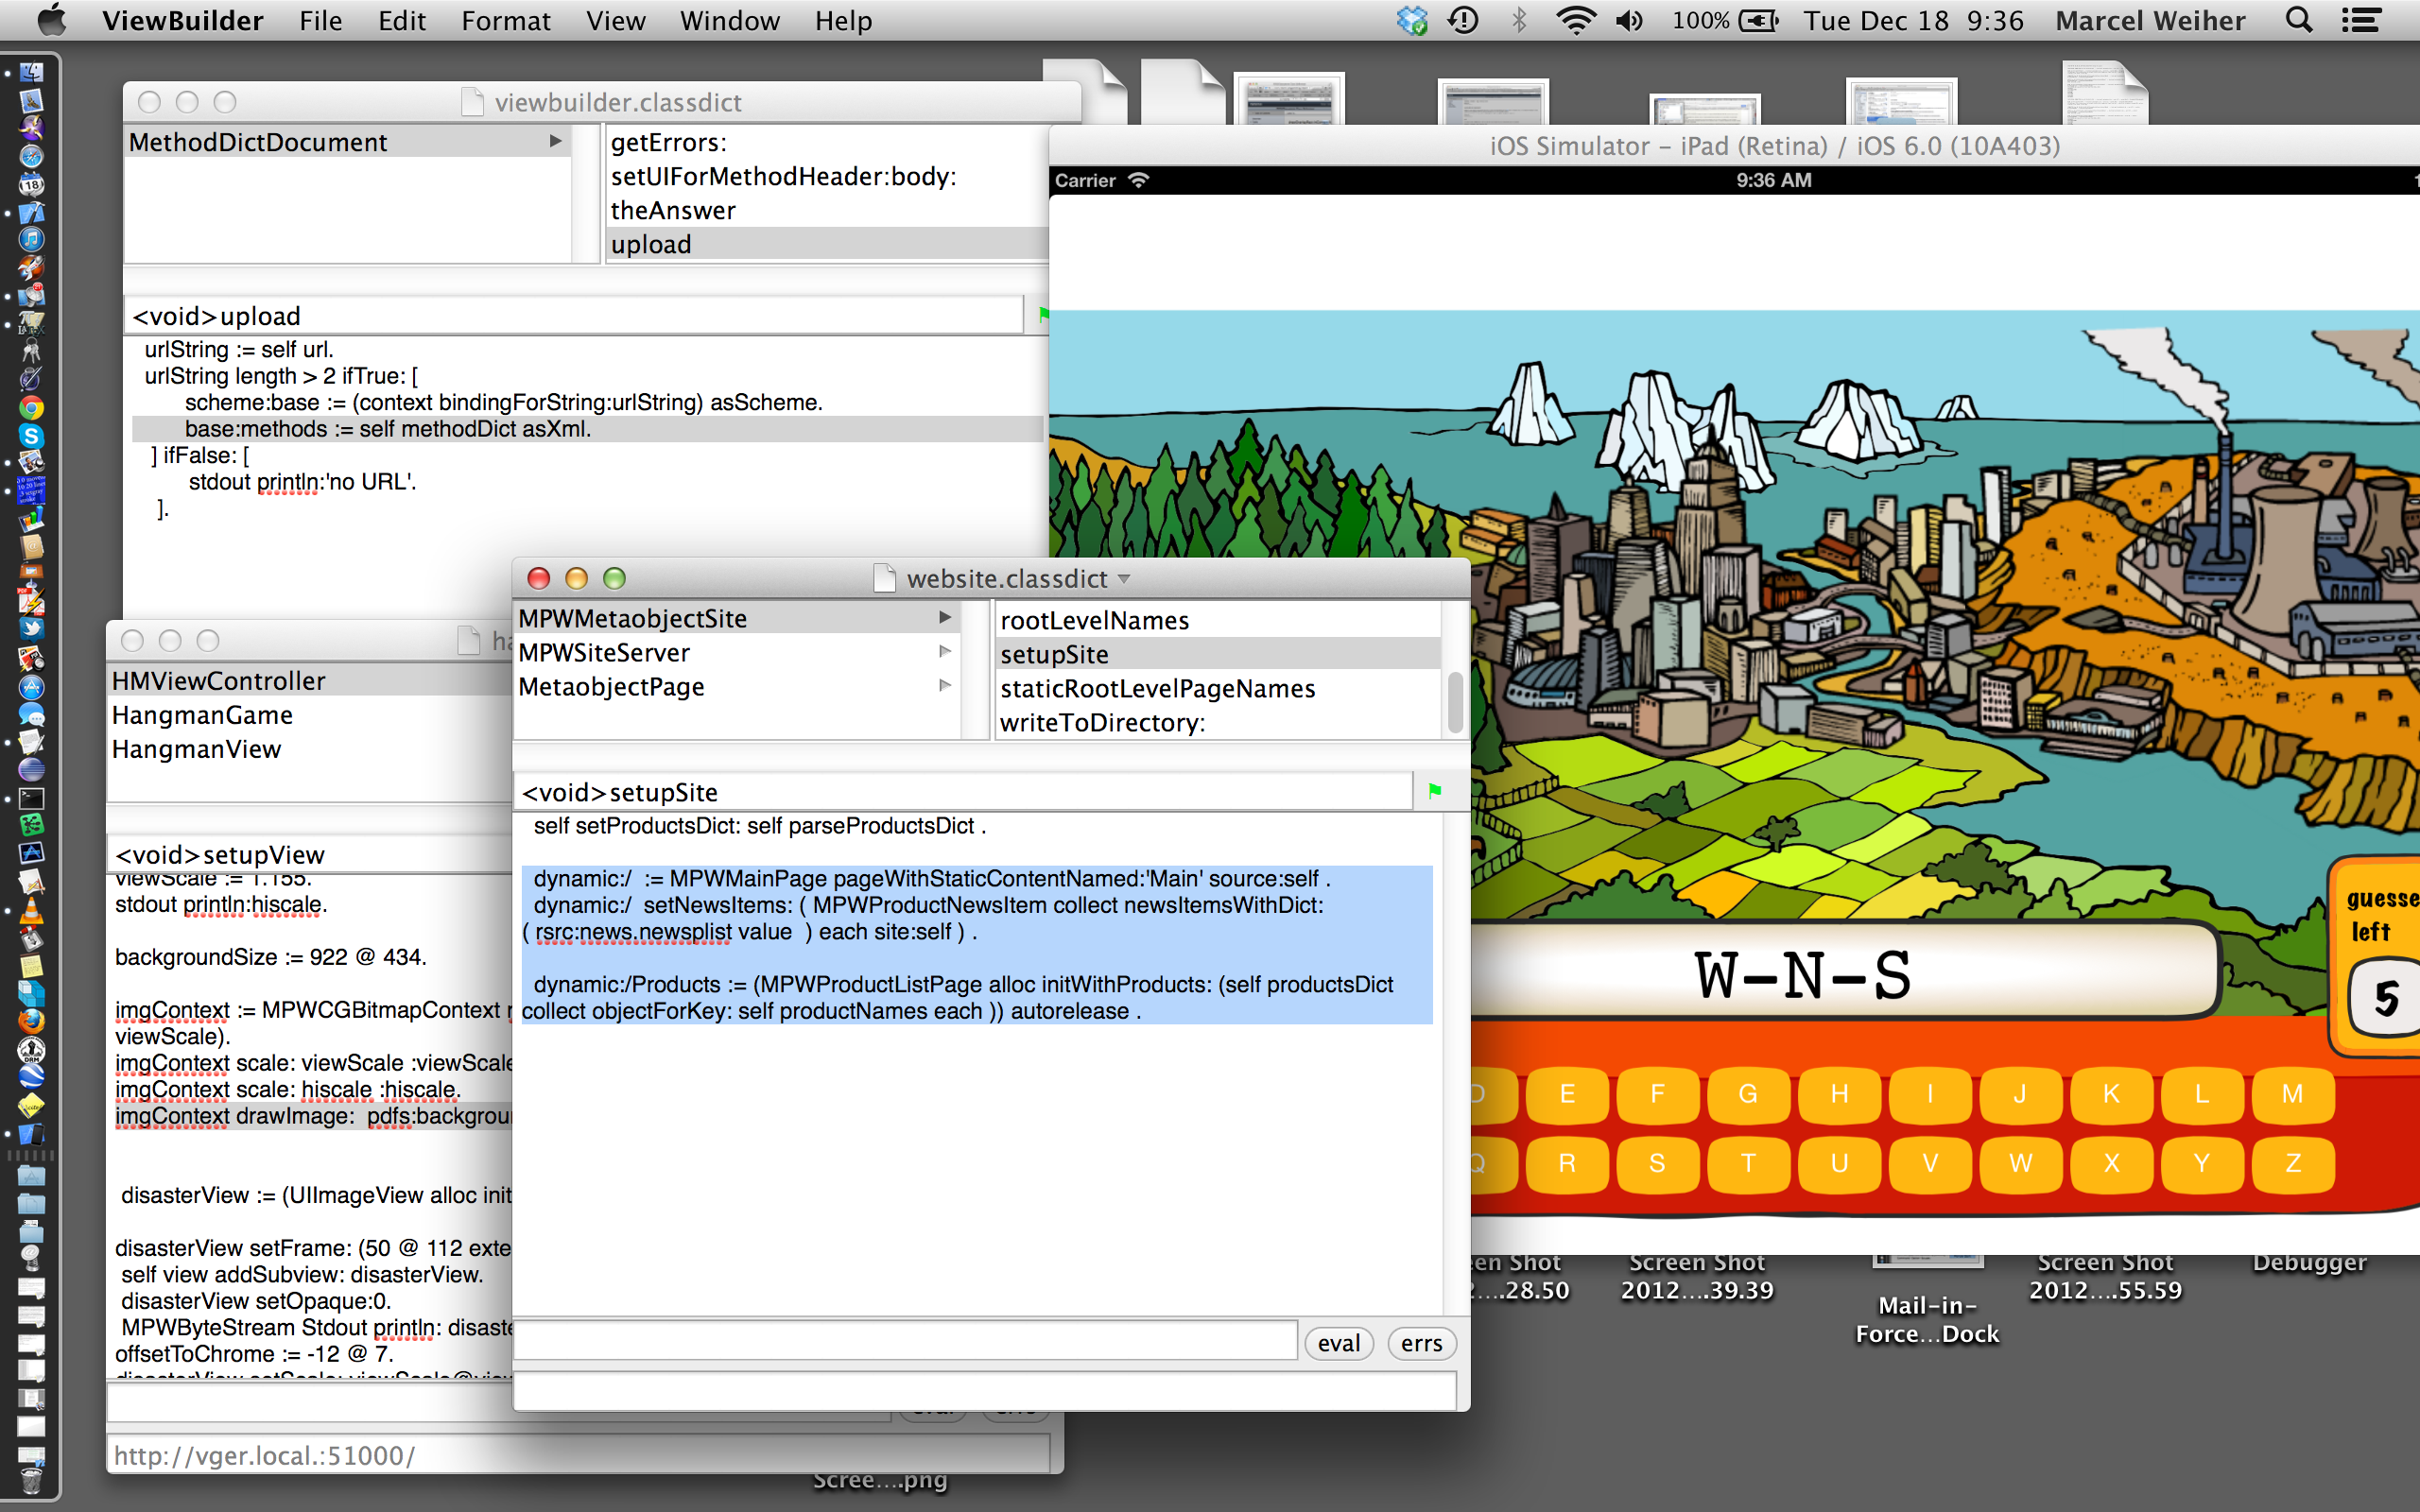
\includegraphics[scale=0.50,page=1]{PolymorphicIdentifiersInUse.png}
\caption{Polymorphic Identifiers in use}
\label{pi-inuse}
\end{figure*}


The game has a large number of graphical assets that could be used much more simply in code by using special schemes for accessing app
resources, though the overall impact was not very high due to large amounts of layout logic. 
 The IDE was initially completely written in Objective-C, but dealing with remote resources was so cumbersome that
those parts were rewritten using Objective-Smalltalk with Polymorphic Identifiers.

The application that gained most from Polymorphic Identifiers was the site generator:  the asset pipeline consisting of static
content, templating mechanism, dynamic content and a page cache could be directly expressed as a series of connected
scheme-handlers.  The object that dynamically generates the site's root is placed there using the simple assignment: {\tt dynamic:/  := MPWMainPage \dots}.

Fig.~\ref{http-server-speed} shows the results.  Serving a specific directory using a relative scheme parametrized
with the file scheme resulted in a performance level of around 19K requests per second.  Adding the same memory cache
we used for the caching http client scheme improves performance to 23K requests per second and finally exporting a pure
memory scheme yields the best performance at 31K requests per second.   Apache has many more features and so
has slightly lower performance.

\begin{figure}
\begin{minipage}[c]{0.58\textwidth}
\begin{tabular}{|l|c|c|} \hline
Server   &  Requests/s    \\ \hline
apache & 	14876	      \\ % \hline
home-scheme (file+relative) &  19231   \\ % \hline
home-scheme (+cached)  &  23398  \\ % \hline
memory-scheme (only) &  31491  \\ \hline
\end{tabular}
\end{minipage}
\begin{minipage}[c]{0.58\textwidth}
\includegraphics[scale=0.38,page=2]{server-perf.pdf}
\end{minipage}
\vspace{-2.0em}
\caption{Performance of different schemes bridged to http vs. apache}
\label{http-server-speed}
\end{figure}



%-=-=-=-=-=-=-=-=-=-=-=-=-=-=-=-=-=-=-=-=-=-=-=-=-=-=-=-=-=-=-=-=-=-=-=%


\section{Related Work}
\label{related-work}


We already saw in section~\ref{direct-reference} that messaging can be used for resource
access in lieu of plain identifiers.  Self~\cite{UngarS87} and Newspeak~\cite{Bracha:2010:MON:1883978.1884007} take this
approach to its logical conclusion by making all identifiers message-sends and therefore late-bound, eliminating
all nouns and replacing them with verbs\footnote{Literals are the exception}.  Although
this elimination of variables as a simplification is conceptually elegant, it leads to problems of scattering and tangling of code we
mentioned, and  ``left a complexity that bothers us to this day''~\cite{Ungar:2007:SEL:1238844.1238853}.
Handling the assignment part of resource access leads to ad-hoc rules and mechanisms to tie together
the slot accessor methods that Ungar and Smith say ``troubled us a bit''~\cite{Ungar:2007:SEL:1238844.1238853}.

Polymorphic Identifiers are a result of the same basic premise that identifiers should always be late-bound.  However,
it doesn't follow the apparent implicit assumption that only messaging can be late-bound and therefore identifiers must
be messages in order to be late-bound, and the related assumption that interfaces must be message-based.

This assumption certainly doesn't apply to the World Wide Web and the REST architectural style~\cite{fielding-rest}, where
it is (universal) resource identifiers that are the interfaces, and messaging is the hidden implementation detail.  This 
approach is taken to its logical extreme by  by Resource Oriented Computing~\cite{roc},
which encodes all computation into identifiers, with an {\tt action:} scheme that is ``a functional programming language encoded as a URI''.

Although scheme-handlers can be exported via http, Polymorphic Identifiers leave the decision of whether to present a messaging
or a resource-based interface to the developers,
similar to properties in C\#~\cite{Archer:2001:IC:516715} and Objective-C 2.0~\cite{Kochan:2009:PO:1538451}, which closely match the proposal in~\cite{Spinellis:2002:MPC:510857.510868}.  Properties are syntactic sugar for a pair of accessor methods and allow clients to use 
 plain identifiers syntax to access values via message-sends, including assignment for setting the value.   However, properties
 are just syntactic sugar for one type of resource access, they are not user-extensible like Polymorphic Identifiers 
 and don't integrate access to external resources or first class references.

Common LISP~\cite{Steele:1990:CLL:95411} has {\tt symbol-macrolet}, which was explicitly limited to lexical scoping due to fears 
that having simple identifiers with overloaded meaning could be confusing~\cite{gabriel-lisp-identifiers}, echoing similar concerns by the creators
of Smalltalk-72 of syntax that was too flexible~\cite{Kay:1996:EHS:234286.1057828}.  Having clear syntactic markers in the form of scheme-prefixes
and directly associating each prefix with one scheme-handler in Polymorphic Identifiers avoids confusion as to the meaning of specific identifiers.

The E language~\cite{MillerRobustComposition}  supports URI-Expressions as a direct language feature using angle brackets for access to 
resources such as files using and to the underlying Java classes:   {\tt $\langle$file:/home/marcs/myFile.txt$\rangle$},  \\ {\tt $\langle$unsafe:java.util.makeCalendar>.getYEAR()$\rangle$}.

E even allows custom schemes to be defined, but  only for read-access, separate from other identifiers and without the ability to extract references.

A different approach to resource access comes from the operating system community:  Plan9 
integrates a wide variety of local and remote~\cite{plan9network} resources and services into a single directory tree~\cite{plan9names} that is made available on a per-process basis, but mediated by the kernel and accessed only indirectly via system calls and string-based
identifiers.
User level filesystems like FUSE~\cite{fuse} or the BSD Pass-to-User-Space~\cite{kantee:puffs} 
system bring some of these ideas to commercial operating systems, but make these filesystems visible globally to all
processes on a machines. 


Polymorphic Identifiers are similar to Embedded Domain Specific Languages~\cite{edsl}
in that they allow domain-specific language elements to be added to a language, rather
than having to create a completely new language with an external DSL or attempt to 
achieve the desired effect with an internal DSL\cite{fowlerdsl}.  

Like polymorphic embedding of DSLs~\cite{polydsl}, Polymorphic Identifiers allow
a single syntax to be used with multiple, pluggable semantic interpretations permitting
composition of functionality~\cite{embeddeddsl}.  However, Polymorphic Identifiers
are applicable to general purpose programming languages, not just DSLs, while
at the same time restricting their focus to the identifiers used.




%-=-=-=-=-=-=-=-=-=-=-=-=-=-=-=-=-=-=-=-=-=-=-=-=-=-=-=-=-=-=-=-=-=-=-=%

\section{Summary and Outlook}
\label{summary-and-outlook}

We have created Polymorphic Identifiers, a generalization of identifiers based on URI
syntax and extensible, pluggable semantics based on scheme-handlers.   
Polymorphic Identifiers allow any type of resource that can be addressed via URI
to be directly referenced, avoiding the need to create and use string-based identifiers 
to access these resources, and providing compiler support for these identifiers.

The uniformity of the syntax and the use of common interfaces for scheme-handlers
enables polymorphic behavior for resource access, permitting different scheme-handlers
to be substituted without affecting client code. Application-specific schemes
enable abstraction.
Custom scheme-handlers can be implemented as normal objects and added
to the language, or even composed from pre-existing handlers and
combinators.

With the user-extensible identifier architecture of Polymorphic Identifiers, it becomes possible to add abstraction
and information-hiding capabilities to identifiers and expand the use of REST-style
programming beyond network and Web-environments.



%\section*{Acknowledgements}

%The authors would like to thank Carl Friedrich Bolz, Gilad Bracha, Richard Gabriel, and Michael Perscheid for their
%helpful feedback.

%-=-=-=-=-=-=-=-=-=-=-=-=-=-=-=-=-=-=-=-=-=-=-=-=-=-=-=-=-=-=-=-=-=-=-=%

%\appendix
%\section{Appendix A}

%This is the text of the appendix, if you need one.

%\acks

%Acknowledgments, if needed.

% We recommend abbrvnat bibliography style.

\vfill
\break

\bibliographystyle{abbrvnat}
\bibliography{polymorphic-identifiers}


% The bibliography should be embedded for final submission.

\balancecolumns

\end{document}
